 \providecommand{\main}{../../..}
\documentclass[\main/main.tex]{subfiles}
\begin{document}
\subsection{Esercizio 4}
Dato il seguente problema di PLI:

\begin{figure}
  \begin{align*}
    \min z =-2x_1+ x_2             \\
    x_1 + x_2   & \leq 4           \\
    6x_1 - 4x_2 & \leq 9           \\
    \bmx        & \in \mathbb{N}^2
  \end{align*}
  \caption{Esercizio 4}
\end{figure}

\begin{table}
  \begin{tabular}{LLLL|L}
    0 & 0 & \sfrac{1}{5} & \sfrac{3}{10}  & -4           \\
    \hline
    1 & 0 & \sfrac{2}{5} & \sfrac{1}{10}  & \sfrac{5}{2} \\
    0 & 1 & \sfrac{3}{5} & \sfrac{-1}{10} & \sfrac{3}{2}
  \end{tabular}
\end{table}

\begin{enumerate}
  \item Si ricavi un taglio di Gomory dal primo vincolo.
  \item Si disegni la regione ammissibile del rilassamento continuo del problema, i punti (più significativi) a coordinate intere interni ad essa ed il taglio generato.
  \item Si riporti il tableau dopo l'inserimento del nuovo vincolo e si indichi l'elemento di pivot individuato dal simplesso duale (non si richiede di effettuare il passo di pivot).
\end{enumerate}

\subsection{Soluzione esercizio 4}
\subsubsection*{Taglio di gomory}
\[
  \gmr{1}x_1+\gmr{\frac{2}{5}}x_3 + \gmr{\frac{1}{10}}x_4 \geq \gmr{\frac{1}{2}}
  \Rightarrow
  \frac{2}{5}x_3 + \frac{1}{10}x_4 \geq \frac{1}{2}
\]
\subsubsection*{Regione ammissibile}
\[
  \begin{cases}
    x_1+x_2+x_3=4   \\
    6x_1-4x_2+x_4=9 \\
    \frac{2}{5}x_3 + \frac{1}{10}x_4 \geq \frac{1}{2}
  \end{cases}
  \Rightarrow
  \begin{cases}
    x_3=4-x_1-x_2   \\
    x_4=9-6x_1+4x_2 \\
    \frac{2}{5}(4-x_1-x_2) + \frac{1}{10}(9-6x_1+4x_2) \geq \frac{1}{2}
  \end{cases}
  \Rightarrow
  x_1 \leq 2
\]

Il vincolo in funzione delle variabili in base risulta quindi:

\[
  x_1 \leq 2
\]

\begin{figure}
  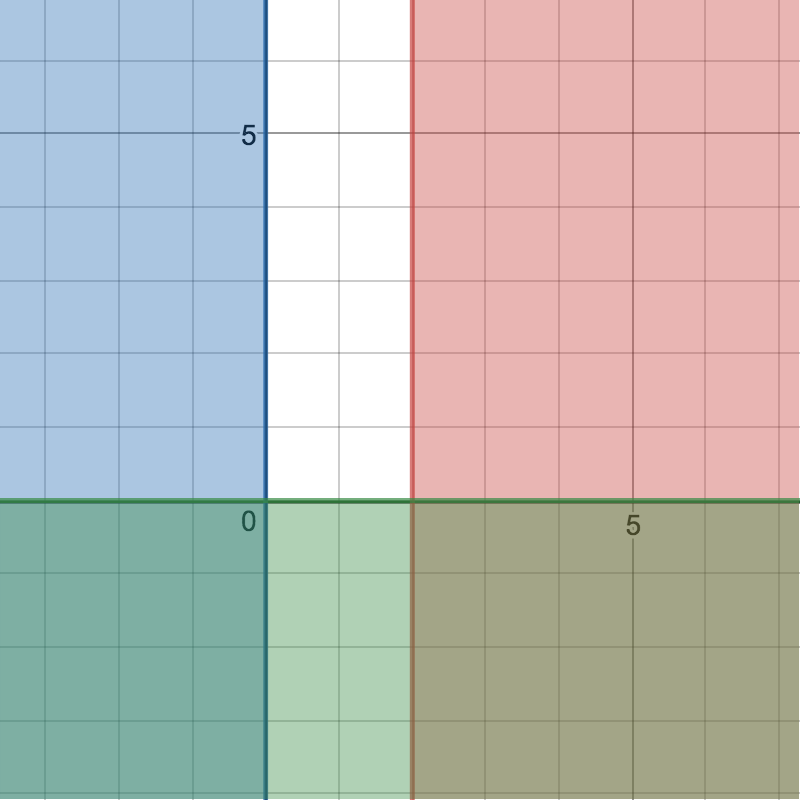
\includegraphics[width=0.4\textwidth]{2015_06_19_04}
\end{figure}

\subsubsection*{Elemento di pivot}
L'elemento scelto è $\sfrac{-2}{5}$, elemento tale per cui $\min\crl{\frac{c_j}{\abs{a_{hj}}}:a_{hj}<0}$.
\begin{table}
  \begin{tabular}{LLLLL|L}
    0 & 0 & \sfrac{1}{5}                      & \sfrac{3}{10}  & 0 & -4            \\
    \hline
    1 & 0 & \sfrac{2}{5}                      & \sfrac{1}{10}  & 0 & \sfrac{5}{2}  \\
    0 & 1 & \sfrac{3}{5}                      & \sfrac{-1}{10} & 0 & \sfrac{3}{2}  \\
    0 & 0 & \cellcolor{green!30}-\sfrac{2}{5} & -\sfrac{1}{10} & 1 & -\sfrac{1}{2}
  \end{tabular}
\end{table}

\end{document}